        \chapter{Chapitre 1 : Cadre général du projet}
        \begin{spacing}{1.2}
        \minitoc
            \thispagestyle{MyStyle}
        \end{spacing}
        \clearpage
        
        \section*{Introduction}
        Dans ce chapitre, nous présentons le cadre général de notre projet de stage. Nous commençons par introduire l’entreprise d’accueil, \textbf{Talan Tunisie Consulting}, ainsi que ses principaux domaines d’activité. Ensuite, nous présentons l’environnement d’innovation dans lequel le projet a été réalisé, à travers \textbf{Talan Innovation Factory}, puis le programme de formation \textbf{BootCamp} suivi au début du stage. Cette partie permet de situer notre travail dans son contexte professionnel, technologique et organisationnel.
        
        \section{L’entreprise d’accueil}

        Cette section présente l’entreprise d’accueil au sein de laquelle s’est déroulé notre stage, à savoir \textbf{Talan Tunisie Consulting}. Nous introduisons également ses principaux domaines d’activité, le cadre d’innovation dans lequel notre projet a été réalisé, ainsi que le programme de formation suivi au début du stage.
        \subsection{Talan Tunisie Consulting}
        
        \begin{figure}[H]
            \centering
            \includegraphics[width=0.35\linewidth]{Logo_Talan.png}
            \caption{Logo de Talan}
            \label{fig:talan_logo}
        \end{figure}
        
        Talan Tunisie Consulting constitue l’implantation tunisienne du groupe \textbf{Talan}, un groupe international de conseil et d’expertises technologiques spécialisé dans la transformation digitale, l’innovation et l’accompagnement des entreprises dans leurs projets à forte valeur ajoutée. Grâce à son expertise multidisciplinaire, Talan accompagne ses clients dans la modernisation de leurs processus métiers, l’intégration de nouvelles technologies et le développement de solutions innovantes.
        
        \subsection{Domaines d’activité}

        Le groupe Talan intervient dans plusieurs secteurs d’activité stratégiques, tels que la finance, l’assurance, l’énergie, le transport et la logistique, les télécommunications, l’industrie ainsi que les services publics. Cette diversité sectorielle lui permet de proposer des solutions adaptées à des besoins métiers variés et d’accompagner les entreprises dans leur transformation numérique.
        
        En parallèle, Talan développe des expertises technologiques transversales dans plusieurs domaines, notamment la \textbf{data}, l’\textbf{intelligence artificielle}, le \textbf{cloud}, la \textbf{cybersécurité}, l’\textbf{automatisation}, ainsi que le développement d’applications et de plateformes numériques. Cette complémentarité entre expertise métier et maîtrise technologique constitue l’un des principaux atouts du groupe.
        
        \subsection{Talan Innovation Factory}
        
        Notre stage s’est déroulé dans un environnement fortement orienté vers l’innovation, représenté par \textbf{Talan Innovation Factory}. Cette entité constitue un espace dédié à la recherche, à l’expérimentation et au développement de solutions innovantes fondées sur les technologies émergentes.
        
        Talan Innovation Factory joue un rôle important dans la valorisation des nouvelles approches technologiques, notamment dans les domaines de l’intelligence artificielle, de la vision par ordinateur, du traitement du langage naturel, des systèmes intelligents et, plus généralement, de la transformation digitale. Elle offre ainsi aux stagiaires et aux ingénieurs un cadre propice à la conception de projets innovants répondant à des problématiques concrètes du monde professionnel.
        
        C’est dans ce contexte que s’inscrit notre projet, qui porte sur le développement d’une solution intelligente d’automatisation des entretiens RH grâce à l’intelligence artificielle générative, à l’analyse multimodale et à l’évaluation intelligente des candidats.

        \subsection{Programme de formation Bootcamp}

        Afin d’aider les stagiaires à acquérir les bases nécessaires à la réalisation de leurs projets, un programme de formation intensif, sous forme de \textbf{bootcamp}, a été organisé durant les premières semaines du stage. Chaque semaine était consacrée à une thématique précise, combinant apprentissage théorique, étude de concepts avancés et mise en pratique à travers des cas d’usage concrets. Cette phase a joué un rôle essentiel dans le renforcement de nos compétences techniques et dans notre préparation au projet de stage.
        
        \begin{itemize}
            \item \textbf{Semaine 1 : Fondements de l’IA, du Machine Learning et du Deep Learning}
        
            Durant cette première semaine, nous avons étudié les notions fondamentales de l’intelligence artificielle, du machine learning et du deep learning. Nous avons également abordé les méthodologies de gestion de projets IA, la collecte et le prétraitement des données, le benchmarking des algorithmes ainsi que les aspects éthiques et réglementaires liés à l’IA. Cette semaine s’est accompagnée d’un mini-projet pratique permettant de mettre en œuvre un cas d’usage de bout en bout.
        
            \item \textbf{Semaine 2 : NLP et Large Language Models}
        
            La deuxième semaine a été consacrée au traitement automatique du langage naturel (\textit{Natural Language Processing}) et aux grands modèles de langage. Nous avons étudié les concepts de base du NLP, les transformers, les mécanismes d’attention, ainsi que les différentes architectures des LLMs. Nous avons également découvert des approches pratiques telles que le \textit{prompt engineering}, le \textit{fine-tuning} et les systèmes de type RAG. Cette partie s’est conclue par la réalisation d’un projet pratique basé sur un modèle de langage.
        
            \item \textbf{Semaine 3 : Systèmes agentiques et multi-agents}
        
            Au cours de cette semaine, nous avons exploré les systèmes agentiques ainsi que les architectures multi-agents. L’objectif était de comprendre comment concevoir des agents intelligents capables de raisonner, de planifier, d’utiliser des outils et de collaborer entre eux au sein d’un même système. Nous avons également étudié des concepts comme l’Agentic RAG, l’intégration MCP, ainsi que des frameworks tels que LangChain, LangGraph et CrewAI. Une attention particulière a été accordée à l’architecture logicielle, à la sécurité et aux bonnes pratiques de développement.
        
            \item \textbf{Semaine 4 : Blockchain et Quantum Computing}
        
            La quatrième semaine a permis d’élargir notre champ d’apprentissage vers deux domaines avancés, à savoir la blockchain et l’informatique quantique, avec un accent particulier sur leur relation avec l’intelligence artificielle. Selon les spécialités, les stagiaires ont suivi un parcours orienté soit vers la blockchain, soit vers le quantum computing. Cette semaine a constitué une opportunité pour découvrir de nouveaux domaines technologiques et enrichir notre vision des innovations émergentes.
        \end{itemize}
        \section{Présentation du projet}

Dans cette section, nous présentons le contexte général du projet ainsi que la problématique à laquelle il répond. Nous décrivons également les principaux objectifs visés par ce travail. Ce projet s’inscrit dans le domaine de l’intelligence artificielle appliquée au recrutement et vise à améliorer certaines étapes du processus de sélection des candidats grâce à l’automatisation et à l’analyse intelligente des entretiens.

\subsection{Problématique}

Le processus de recrutement constitue une étape essentielle pour les entreprises souhaitant identifier les candidats les plus adaptés à leurs besoins. Cependant, ce processus peut être long et exige souvent une mobilisation importante de ressources humaines, notamment lors de l’analyse des candidatures, de la présélection des profils et de la conduite des entretiens.

Dans de nombreux cas, les recruteurs doivent traiter un grand nombre de candidatures dans un délai limité, ce qui peut rendre difficile l’évaluation objective et cohérente des candidats. De plus, certaines compétences telles que la communication, la capacité d’analyse ou la résolution de problèmes sont parfois difficiles à évaluer uniquement à partir du CV.

Face à ces défis, l’intégration de solutions basées sur l’intelligence artificielle peut contribuer à améliorer l’efficacité du processus de recrutement. L’utilisation d’un système intelligent capable de générer des questions d’entretien, d’analyser les réponses des candidats et de fournir une évaluation automatisée représente une approche innovante pour assister les recruteurs dans leur prise de décision.

\subsection{Objectifs}

L’objectif principal de ce projet est de concevoir et de développer une plateforme intelligente permettant d’automatiser certaines étapes du processus de recrutement à l’aide de technologies d’intelligence artificielle.

Plus précisément, ce projet vise à :

\begin{itemize}
    \item Générer automatiquement des questions d’entretien adaptées au poste et au profil du candidat.
    
    \item Mettre en place un système d’entretien automatisé permettant d’interagir avec les candidats.
    
    \item Analyser les réponses des candidats afin d’évaluer leurs compétences techniques et comportementales.
    
    \item Fournir un score ou un rapport d’évaluation permettant d’aider les recruteurs dans la sélection des candidats.
    
    \item Offrir aux candidats la possibilité de réaliser des entretiens simulés afin de se préparer avant un entretien réel.
\end{itemize}

Ainsi, cette solution vise à améliorer l’efficacité et la rapidité du processus de recrutement tout en offrant une expérience interactive et innovante pour les candidats et les recruteurs.
\section{Étude de l’existant}

L’analyse de l’existant constitue une étape importante dans le développement de notre projet. Elle permet d’identifier les solutions déjà proposées sur le marché, d’analyser leurs fonctionnalités principales ainsi que leurs avantages et leurs limites. Cette étude nous aide à mieux comprendre les technologies utilisées dans le domaine du recrutement intelligent et à définir les améliorations que notre solution peut apporter.

Dans ce cadre, nous avons sélectionné trois plateformes utilisant l’intelligence artificielle dans le processus de recrutement : \textbf{HireVue}, \textbf{Pymetrics} et \textbf{Talview}.

\subsection{Étude de l’application « HireVue »}

\textbf{1. Description :}

HireVue est une plateforme de recrutement basée sur l’intelligence artificielle qui permet aux entreprises de réaliser des entretiens vidéo automatisés. La solution analyse les réponses des candidats à travers des technologies d’analyse vidéo, de traitement du langage naturel et d’évaluation comportementale. Elle permet ainsi aux recruteurs de gagner du temps lors de la phase de présélection des candidats.

\begin{figure}[H]
\centering
\includegraphics[width=0.3\linewidth]{hirevue.png}
\caption{Interface de la plateforme HireVue}
\end{figure}

\textbf{2. Avantages et limites :}

\begin{table}[H]
\centering
\begin{tabular}{|p{6cm}|p{6cm}|}
\hline
\textbf{Avantages} & \textbf{Limites} \\
\hline
Automatisation des entretiens vidéo permettant un gain de temps pour les recruteurs. & L’analyse automatisée peut parfois manquer de transparence dans les critères d’évaluation. \\
\hline
Utilisation de l’intelligence artificielle pour analyser les réponses des candidats. & Certaines personnes peuvent se sentir mal à l’aise lors d’un entretien automatisé. \\
\hline
Possibilité d’évaluer plusieurs candidats simultanément. & Risque de biais algorithmiques si les données d’entraînement ne sont pas équilibrées. \\
\hline
\end{tabular}
\caption{Avantages et limites de HireVue}
\end{table}


\subsection{Étude de l’application « Vervoe »}

\textbf{1. Description :}

Vervoe est une plateforme de recrutement intelligente basée sur l’évaluation des compétences réelles des candidats à travers des tests personnalisés et des simulations de travail.
La plateforme utilise l’intelligence artificielle pour analyser automatiquement les réponses des candidats, évaluer leurs performances et classer les profils selon leur adéquation avec le poste proposé.
Vervoe permet ainsi aux recruteurs de gagner du temps tout en améliorant la précision du processus de sélection.

\begin{figure}[H]
\centering

\includegraphics[width=0.3\linewidth]{vervoe.png}
\caption{Interface de la plateforme vervoe}
\end{figure}

\textbf{2. Avantages et limites :}

\begin{table}[H]
\centering
\begin{tabular}{|p{6cm}|p{6cm}|}
\hline
\textbf{Avantages} & \textbf{Limites} \\
\hline
Évaluation des candidats à travers des mises en situation et des tests pratiques. & Les évaluations peuvent être longues selon le type de poste. \\
\hline
Automatisation du classement des candidats grâce à l’intelligence artificielle. & Nécessite une connexion Internet stable et un bon équipement. \\
\hline
Réduction du temps de recrutement et amélioration de l’expérience candidat. & Certains aspects humains et comportementaux peuvent être difficiles à évaluer automatiquement. \\
\hline
\end{tabular}
\caption{Avantages et limites de Vervoe}
\end{table}


\subsection{Étude de l’application « Talview »}

\textbf{1. Description :}

Talview est une plateforme de recrutement intelligente qui permet d’organiser des entretiens vidéo automatisés, des évaluations en ligne et des tests techniques. Elle utilise l’intelligence artificielle pour analyser les performances des candidats et fournir aux recruteurs des rapports détaillés facilitant la prise de décision.

\begin{figure}[H]
\centering
\includegraphics[width=0.3\linewidth]{talview.png}
\caption{Interface de la plateforme Talview}
\end{figure}

\textbf{2. Avantages et limites :}

\begin{table}[H]
\centering
\begin{tabular}{|p{6cm}|p{6cm}|}
\hline
\textbf{Avantages} & \textbf{Limites} \\
\hline
Plateforme complète intégrant entretiens vidéo et tests techniques. & Dépend fortement de la qualité de la connexion internet. \\
\hline
Analyse automatisée des performances des candidats. & Certaines fonctionnalités avancées nécessitent un abonnement payant. \\
\hline
Facilite la gestion d’un grand nombre de candidatures. & Peut nécessiter une formation initiale pour les recruteurs. \\
\hline
\end{tabular}
\caption{Avantages et limites de Talview}
\end{table}
\subsection{Étude de l’application « Asendia AI »}

\textbf{1. Description :}

Asendia AI est une plateforme d’entretien intelligent basée sur l’intelligence artificielle conversationnelle. 
Elle permet de réaliser des entretiens adaptatifs et d’analyser les réponses des candidats afin de fournir un feedback comportemental détaillé. 
La plateforme vise à améliorer l’expérience candidat tout en aidant les recruteurs à mieux comprendre les compétences comportementales et communicationnelles des postulants.

\begin{figure}[H]
\centering
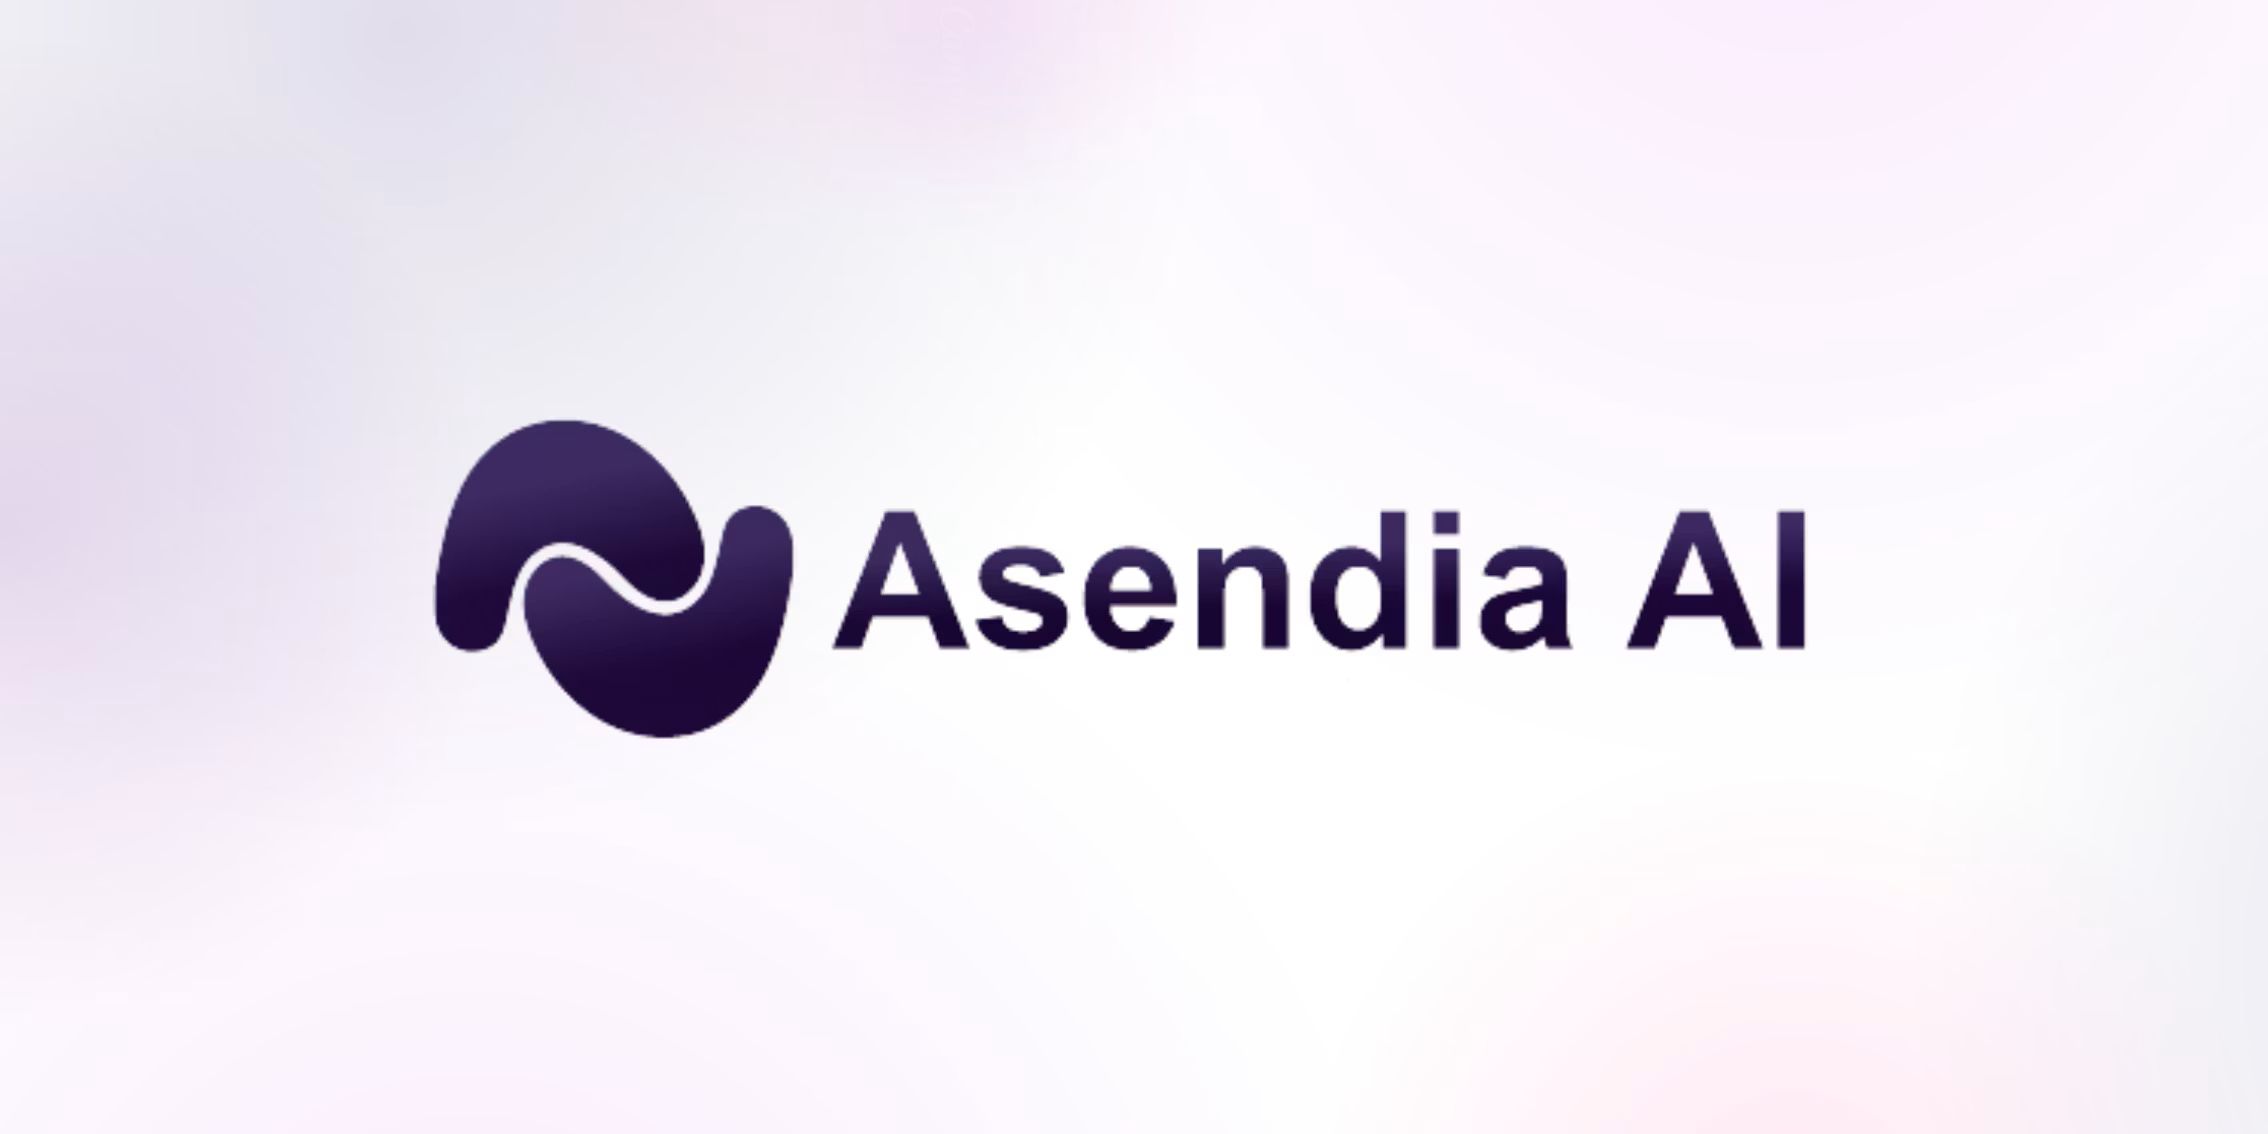
\includegraphics[width=0.4\textwidth]{images/asendia.png}
\caption{Interface de la plateforme Asendia AI}
\label{fig:asendia}
\end{figure}

\textbf{2. Avantages et limites :}

\begin{table}[H]
\centering
\begin{tabular}{|p{6cm}|p{6cm}|}
\hline
\textbf{Avantages} & \textbf{Limites} \\
\hline
Bonne IA conversationnelle pour les entretiens adaptatifs. & Pas d’analyse vidéo par IA. \\
\hline
Fournit un feedback comportemental détaillé. & Pas d’analyse multimodale avancée. \\
\hline
Améliore l’interaction et l’expérience candidat. & Pas d’évaluation technique des compétences. \\
\hline
Ne couvre pas uniquement les entretiens classiques. & Ne couvre pas l’ensemble du processus de recrutement. \\
\hline
\end{tabular}
\caption{Avantages et limites de Asendia AI}
\label{tab:asendia}
\end{table}

\subsection{Limites des solutions existantes}

Bien que ces outils soient performants, ils présentent encore de nombreuses limites. Ce sont d’ailleurs ces limites qui ont motivé la conception de notre propre solution.

% TODO : remplacer les renvois [24, 18] et [25] par de vraies entrées \cite{} dans chapitre/09-Bibliographie.tex
\begin{itemize}
    \item \textbf{Biais et équité :} les modèles d’intelligence artificielle apprennent à partir de données historiques ; ils risquent donc de reproduire les décisions injustes prises auparavant par les recruteurs humains. Un candidat ayant un accent prononcé, issu d’une culture différente ou présentant un mode de communication neuro-atypique peut ainsi obtenir un score plus faible, alors même qu’il correspond parfaitement au poste [24, 18].

    \item \textbf{Faible prise en charge des langues locales :} la plupart de ces plateformes sont conçues pour l’anglais ou pour d’autres langues largement répandues. Or, l’arabe ne constitue pas une langue unique : les candidats mêlent fréquemment le dialecte tunisien, le français et l’anglais, et s’expriment parfois en « franco-arabe » (\textit{arabizi}). Lorsque l’IA ne parvient pas à interpréter ce mélange, elle passe à côté du sens réel des réponses et peut attribuer un score erroné [25]. Il s’agit là d’un problème majeur dans le contexte tunisien, qui correspond précisément au cadre de notre projet.

    \item \textbf{Expérience impersonnelle pour le candidat :} beaucoup de ces outils reposent sur la vidéo asynchrone, à sens unique, où le candidat s’adresse uniquement à un écran sans jamais voir un interlocuteur réel. Cette situation peut s’avérer stressante et déshumanisante, et renvoie une image peu valorisante de l’entreprise [25].

    \item \textbf{Absence de vérification :} de nombreux candidats embellissent leurs compétences lors des entretiens. Ainsi, lorsqu’un candidat affirme maîtriser un framework ou une technologie donnée, rien ne permet de garantir la véracité de ses propos, ni qu’il dispose réellement d’une expérience pratique avec ces outils.
\end{itemize}

Ces limites montrent qu’il existe toujours un réel besoin d’un système de recrutement à la fois interactif, capable de comprendre le dialecte tunisien, préservant le confort du candidat grâce à un avatar 3D, tout en demeurant équitable et fiable. C’est précisément cette lacune que notre projet cherche à combler.
\section{Notre solution}

À l'issue de l'étude de l'existant et afin de pallier les limites identifiées dans les solutions actuelles, nous proposons de développer une plateforme intelligente d'automatisation des entretiens RH. Contrairement aux outils existants qui reposent sur une vidéo à sens unique, notre solution conduit un véritable entretien interactif entre le candidat et un intervieweur virtuel animé par l'IA. Elle exploite l'intelligence artificielle générative, l'analyse multimodale et un avatar 3D parlant, tout en intégrant une vérification concrète des compétences techniques et un module de détection de fraude. L'ensemble de la plateforme a été conçu pour répondre aux spécificités du contexte tunisien, notamment la prise en charge du dialecte local et la mixité linguistique des candidats.

\subsection{Fonctionnalités de la solution}

La plateforme repose sur les fonctionnalités clés décrites ci-dessous.

\begin{itemize}
  \item \textbf{Entretien IA interactif} : l'entretien est piloté par un agent qui le découpe en sections, l'ouvre par une question d'accueil personnalisée, puis, à chaque tour, évalue la réponse et décide de la suite : poser une nouvelle question, proposer un exercice de code ou clore l'entretien. Chaque entretien est ainsi dynamique et adapté au candidat, et non une liste figée de questions.

  \item \textbf{Questions fondées sur le CV et sur le poste} : les questions sont générées à partir du CV du candidat et des exigences de l'offre d'emploi, ce qui rend l'entretien pertinent et personnalisé pour chacun.

  \item \textbf{Avatar 3D parlant} : pour mettre le candidat à l'aise et réduire son stress, l'intervieweur prend la forme d'un avatar 3D animé. L'avatar énonce les questions par synthèse vocale (\textit{text-to-speech}, TTS) et le mouvement de ses lèvres est synchronisé avec la voix (\textit{lip-sync}), afin de rendre l'échange plus naturel.

  \item \textbf{Transcription en direct et analyse de la voix} : pendant que le candidat parle, le système retranscrit sa réponse en temps réel et analyse la voix pour en dégager l'émotion et le sentiment. L'évaluation gagne ainsi une dimension multimodale, au-delà du seul texte de la réponse.

  \item \textbf{Vérification réelle des compétences par des exercices de code} : pour pallier le manque de vérification, l'IA peut envoyer un exercice de code au cours de l'entretien. Le candidat écrit du code réel, exécuté de manière sécurisée dans un bac à sable isolé (\textit{sandbox}). Lorsqu'un candidat affirme maîtriser une technologie, le système peut donc le vérifier par une tâche concrète plutôt que de s'en tenir à sa parole.

  \item \textbf{Détection de fraude} : un module distinct surveille la webcam pendant l'entretien pour s'assurer que le candidat est bien la personne attendue et qu'il ne triche pas. Il s'appuie sur la détection de visage, le suivi du regard, la détection de plusieurs visages et la détection d'objets (un téléphone, par exemple), avec une surveillance audio optionnelle. À la fin de l'entretien, un rapport des anomalies, accompagné de captures d'écran, est généré et transmis au recruteur.

  \item \textbf{Enregistrement, notation et relecture pour le recruteur} : le recruteur ne perd plus de temps sur la première présélection. L'entretien est enregistré et noté, les moments où le candidat se distingue étant signalés. Le recruteur peut tout revoir ensuite et saisir rapidement la performance du candidat.

  \item \textbf{Retour pour les deux parties} : à l'issue de l'entretien, le système fournit un retour au candidat sur sa prestation, et au recruteur pour l'aider à décider mieux et plus vite.

  \item \textbf{Recommandation d'offres} : la plateforme recommande aussi au candidat les offres qui lui correspondent le mieux, à partir de son CV, des descriptions de poste et de sa performance lors de l'entretien.

  \item \textbf{L'humain garde la main} : le système est rapide, équitable et standardisé afin de limiter les biais, mais la décision finale d'embauche revient toujours au recruteur, qui mobilise son expérience et son intuition.
\end{itemize}

En résumé, notre solution réunit dans une seule plateforme un entretien IA interactif, un avatar 3D engageant, une vérification réelle des compétences, la détection de fraude, la notation, le retour d'information et la recommandation d'offres. Elle cherche à conserver la rapidité et le passage à l'échelle d'un outil automatisé tout en restant humaine et équitable envers le candidat.

\section{Méthodologie de travail}

Dans le cadre de ce projet, nous avons adopté la méthodologie Scrum, une approche Agile fondée sur des itérations courtes appelées \textit{sprints}. Cette méthode nous a permis d'organiser le travail de façon progressive, de prioriser les tâches dans un \textit{backlog}, de suivre l'avancement à l'aide de Trello et d'améliorer la solution à chaque étape du développement. À la fin de chaque sprint, nous présentions le résultat à nos encadrantes et ajustions le plan du sprint suivant, ce qui a maintenu une réelle souplesse et nous a permis de réagir vite aux nouveaux besoins comme aux difficultés rencontrées lors de l'intégration des services.

\subsection{Découpage en sprints}

Le développement a été réparti en huit sprints, reconstitués à partir de l'historique de gestion de versions du projet. Le tableau~\ref{tab:sprints} les récapitule.

\begin{table}[ht]
  \centering
  \caption{Sprints du projet reconstitués à partir de l'historique Git}
  \label{tab:sprints}
  \begin{tabular}{@{}p{1.8cm}p{3.2cm}p{8.3cm}@{}}
    \toprule
    \textbf{Sprint} & \textbf{Période (2026)} & \textbf{Objectif principal et livrables} \\
    \midrule
    Sprint 0 & 23 mars               & Initialisation du projet, publication du code source, configuration du dépôt Git, mise en place de la structure initiale du front-end et du back-end. \\[4pt]
    Sprint 1 & 25 mars -- 01 avril   & Développement du système de quiz, sécurisation des quiz, intégration LinkedIn, premières fonctionnalités du workflow recruteur (branche \textit{quiz}). \\[4pt]
    Sprint 2 & 01 avril -- 13 avril  & Module de planification (\textit{scheduling}), première version de la salle d'entretien, intégration du pipeline vocal, amélioration du front-end. \\[4pt]
    Sprint 3 & 13 avril -- 28 avril  & Agent d'entretien vocal, mise à jour de l'interface utilisateur, finalisation du pipeline voix-entretien (branche \textit{scheduling}). \\[4pt]
    Sprint 4 & 28 avril -- 04 mai    & Mises à jour du moteur de salle d'entretien (\textit{callroom}), amélioration du moteur vocal et du flux d'entretien. \\[4pt]
    Sprint 5 & 04 mai -- 21 mai      & Consolidation de la salle d'entretien, stabilisation des fonctionnalités, correctifs et mises à jour utilisateur. \\[4pt]
    Sprint 6 & 21 mai -- 03 juin     & Agent d'entretien dynamique, rapports pondérés, liaison salle d'entretien\,\textrightarrow\,offre d'emploi, corrections d'environnement et de lancement. \\[4pt]
    Sprint 7 & 03 juin -- 31 juillet & Finalisation et déploiement, sécurité et durcissement, rédaction du rapport, préparation de la soutenance. \\
    \bottomrule
  \end{tabular}
\end{table}

\subsection{Planning du projet}

En résumé, la méthodologie Scrum nous a permis de livrer un incrément fonctionnel à chaque sprint et d'affiner progressivement la solution, du premier prototype jusqu'à une plateforme intégrée et déployée.

% ---------------------------------------------------------------
\section{Outils de gestion de projet}

Afin d'assurer le suivi des tâches et la coordination du travail au sein de l'équipe, nous avons eu recours à des outils de gestion de projet adaptés à notre démarche Agile. Ces outils nous ont permis de centraliser les échanges, d'organiser les réunions et de maintenir une communication fluide tout au long du développement.

\subsection{Microsoft Teams}

Microsoft Teams est une application de messagerie et de collaboration développée par Microsoft. Elle facilite la communication au sein d'une équipe en centralisant les discussions, en permettant l'organisation de réunions en ligne et en offrant le partage de documents en temps réel. En réduisant la dépendance aux courriers électroniques, Microsoft Teams contribue à améliorer la productivité globale de l'équipe et à fluidifier les échanges entre les différents membres du projet.

La figure~\ref{fig:teams} illustre l'interface de Microsoft Teams telle qu'elle a été utilisée dans le cadre de notre projet.

\begin{figure}[H]
  \centering
  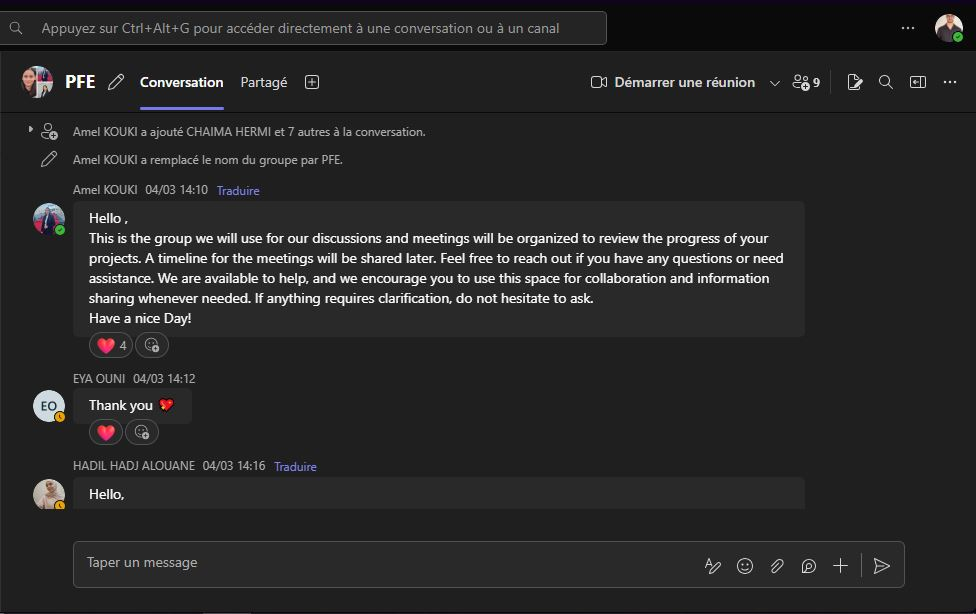
\includegraphics[width=0.85\textwidth]{images/teams.png}
  \caption{Interface de Microsoft Teams utilisée pour la communication et la collaboration.}
  \label{fig:teams}
\end{figure}

% ---------------------------------------------------------------
\section{Diagramme de Gantt}

Un diagramme de Gantt est un outil de planification visuel qui représente le calendrier d'un projet sous forme de barres horizontales. Chaque barre correspond à une tâche ou à un sprint : sa position sur l'axe du temps indique la date de début, sa longueur traduit la durée, et son extrémité droite marque la date de fin prévue. Ce type de diagramme permet d'avoir une vue d'ensemble claire et immédiate de l'enchaînement des activités et de l'état d'avancement du projet.

La figure~\ref{fig:gantt} présente le diagramme de Gantt de notre projet, qui retrace l'enchaînement des huit sprints Agile Scrum, depuis la mise en place initiale jusqu'à la finalisation et au déploiement de la plateforme.

%% Gantt — real sprint dates from git history (Mar 23 – Jul 31 2026 = 19 weeks)
\begin{figure}[H]
\centering
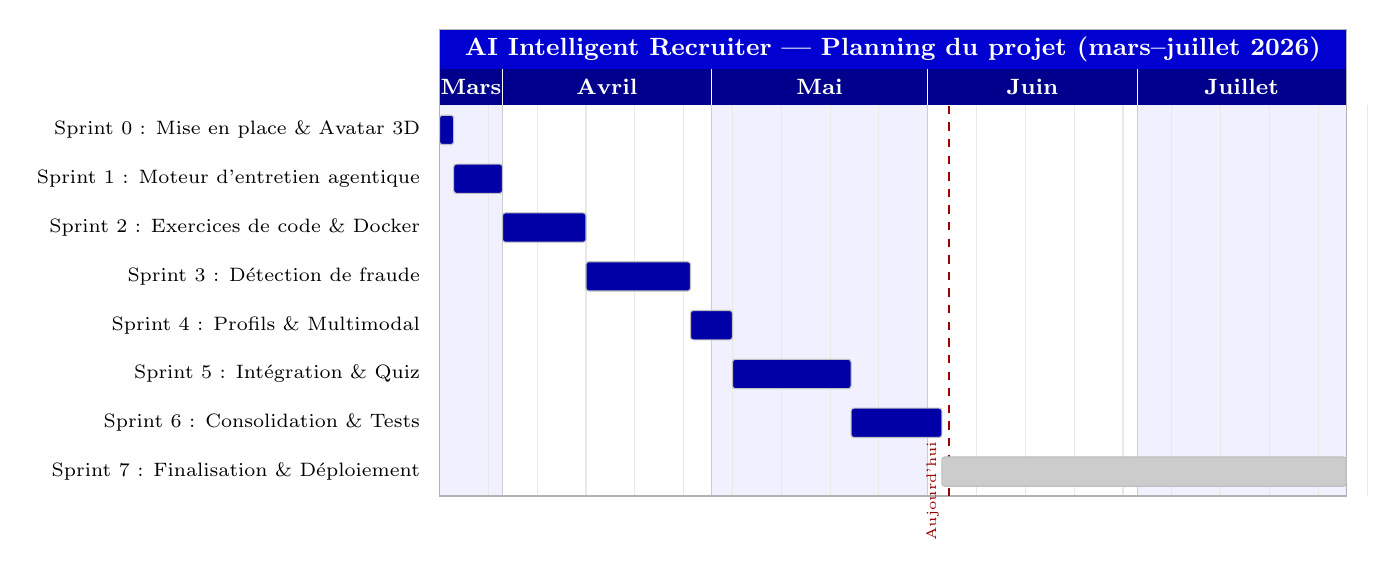
\begin{tikzpicture}[x=0.62cm, y=0.62cm]
  \def\nw{19}
  \def\nr{8}
  \fill[blue!6]  (0,0) rectangle (1.29,\nr);
  \fill[white]   (1.29,0) rectangle (5.57,\nr);
  \fill[blue!6]  (5.57,0) rectangle (10.0,\nr);
  \fill[white]   (10.0,0) rectangle (14.29,\nr);
  \fill[blue!6]  (14.29,0) rectangle (18.57,\nr);
  \foreach \x in {0,1,...,19} { \draw[gray!18] (\x,0) -- (\x,\nr); }
  \fill[blue!82!black] (0,\nr+0.75) rectangle (18.57,\nr+1.55);
  \node[text=white, font=\small\bfseries, anchor=center] at (9.285,\nr+1.15)
    {AI Intelligent Recruiter \textemdash{} Planning du projet (mars\textendash{}juillet 2026)};
  \fill[blue!55!black] (0,\nr) rectangle (18.57,\nr+0.75);
  \foreach \a/\b/\m in {0/1.29/Mars,1.29/5.57/Avril,5.57/10.0/Mai,10.0/14.29/Juin,14.29/18.57/Juillet}{
    \draw[white!50, thin] (\a,\nr) -- (\a,\nr+0.75);
    \node[text=white, font=\footnotesize\bfseries, anchor=center] at ({(\a+\b)/2},\nr+0.375) {\m};
  }
  \draw[white!50, thin] (18.57,\nr) -- (18.57,\nr+0.75);
  \foreach \a in {1.29,5.57,10.0,14.29}{ \draw[gray!40] (\a,0) -- (\a,\nr); }
  \draw[gray!60] (0,0) rectangle (18.57,\nr+1.55);
  \draw[red!60!black, dashed, line width=0.7pt] (10.43,0) -- (10.43,\nr);
  \node[font=\tiny, text=red!60!black, rotate=90, anchor=south] at (10.43,0.1) {Aujourd'hui};
  \foreach \i/\lab/\s/\e/\col in {
    0/{Sprint 0 : Mise en place \& Avatar 3D}/0/0.29/blue!65!black,
    1/{Sprint 1 : Moteur d'entretien agentique}/0.29/1.29/blue!65!black,
    2/{Sprint 2 : Exercices de code \& Docker}/1.29/3.0/blue!65!black,
    3/{Sprint 3 : Détection de fraude}/3.0/5.14/blue!65!black,
    4/{Sprint 4 : Profils \& Multimodal}/5.14/6.0/blue!65!black,
    5/{Sprint 5 : Intégration \& Quiz}/6.0/8.43/blue!65!black,
    6/{Sprint 6 : Consolidation \& Tests}/8.43/10.29/blue!65!black,
    7/{Sprint 7 : Finalisation \& Déploiement}/10.29/18.57/gray!40
  }{
    \pgfmathsetmacro{\yy}{\nr - 0.5 - \i}
    \node[anchor=east, font=\scriptsize] at (-0.2,\yy) {\lab};
    \fill[\col, draw=black!25, thin, rounded corners=1pt] (\s,\yy-0.30) rectangle (\e,\yy+0.30);
  }
\end{tikzpicture}
\caption{Diagramme de Gantt du projet : enchaînement des sprints Agile Scrum (mars--juillet~2026).}
\label{fig:gantt}
\end{figure}

\section{Conclusion}

Ce chapitre a permis de poser le cadre général du projet. Nous avons commencé par présenter l'entreprise d'accueil et ses domaines d'activité. Nous avons ensuite exposé la problématique, analysé les solutions existantes et présenté notre propre solution. Enfin, nous avons décrit la méthodologie adoptée, le découpage en sprints et le planning du projet.

Le chapitre suivant se concentrera sur l'analyse des besoins et la conception de la solution, en présentant les cas d'utilisation, l'architecture générale et les choix technologiques retenus.
